\documentclass[a4paper,12pt]{article}

\usepackage[margin=1in]{geometry}
\usepackage{tikz}
\usepackage{amssymb}
\usepackage{xcolor}
\usepackage{circuitikz}
\usepackage{graphicx}

\newcommand{\ra}{$\rightarrow$}
\newenvironment{6mini}{
  \begin{minipage}{6cm}
}{
  \end{minipage}
}

\title{\texttt{Flipflops}\\\hrulefill}
\author{module 13}
\date{\small{11/12/2023}}

\begin{document}
    \maketitle

    \subsubsection{Latch problems - Continuation}
        The output can respond to any input within an enable is active. This could cause asynchronous behaviour.\\
        \par A solution to this is creating a transition enable (creating \texttt{flipflops})
        \begin{itemize}
        \item Enable is only active when transitioning from active LOW to active HIGH or vice versa
        \item Only register input on clock's edges (rising or falling)
        \end{itemize}
    \section{D flipflop}
        A flip flop has D latch behaviour,but operates on a clock edge.
        \begin{itemize}
            \item Triangles on clock schematics denote a clock input
        \end{itemize}
        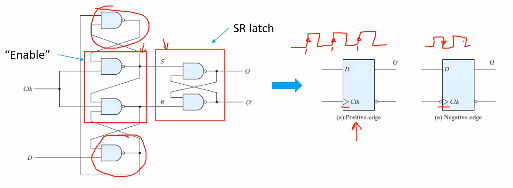
\includegraphics[width=15cm]{DflipflopSchem.png}\\
        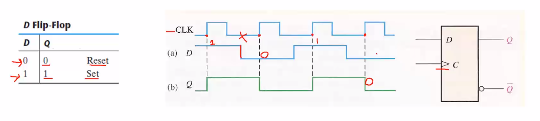
\includegraphics[width=12cm]{DflipflopTime.png}
    \section{JK Flip Flop}
        Equivalent to the SR latch, but edge triggerd and no unstable input condition.
        \begin{itemize}
          \item J is "set"
          \item K is "reset"
        \end{itemize}
         In the case of both inputs being active, the output toggles(compliment).\\
         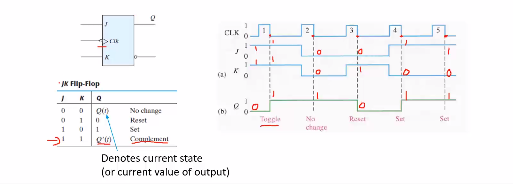
\includegraphics[width=14cm]{JKFlipflopSchem.png}
    \section{T flip Flop}
        \begin{itemize}
          \item Output toggles between HIGH and LOW as long as T is HIGH
        \end{itemize}
        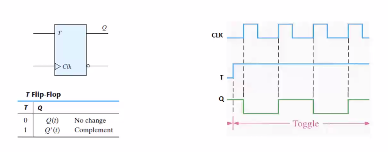
\includegraphics[width=14cm]{TflipFlopSchem.png}
    \section{Making Other Flips Flops from D}
        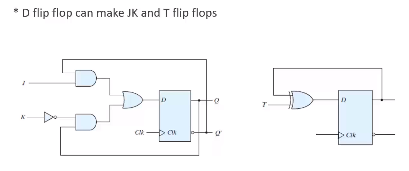
\includegraphics[width=14cm]{DtoTandJK.png}
    \section{Asynchronous Inputs}
        These inputs are not dependent on the clock. As soon as they change, the output is affected.
        \begin{itemize}
          \item They are help to initialize to a given state, or clear to a starting state
          \item Changes output in between clock edges
          \item Typically active low
        \end{itemize}
        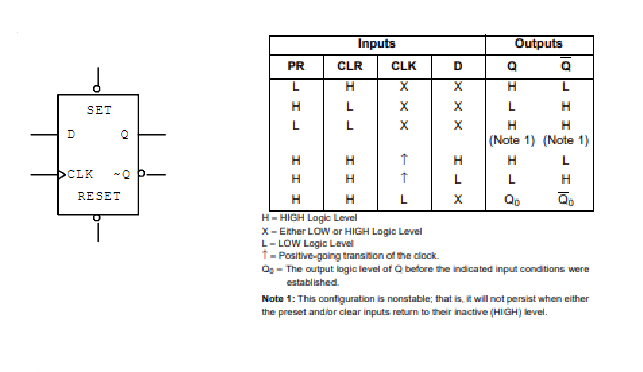
\includegraphics[width=12cm]{AsyncInputs.png}
    \section{Flip Flop Uses}
        The exist as basic storage elements in digital logic
        \begin{itemize}
          \item Counters
          \item Timers
          \item Memory
          \item Timers
          \item Frequency Dividers
          \item Sequential logic circuits
          \item Registers
        \end{itemize}
      \section{Analysis of Sequential Logic Circuits}
        \textbf{State equations} are similar to Boolean expresions from combinational logic \ra~ describe the ouput and transition logic of circuit.\\ \\
        \textbf{State tables} are similar to truth tables \ra~ describe state tramsotopm amdoutput given combination of inputs.\\ \\\textbf{State diagrams} are visual representations of te state table.

        \subsection{Circuit to State Equation}
          State equation is the boolean expression for circuit.\\ \\\textbf{Will have multiple equations}
          \begin{itemize}
            \item One for output of circuit F
            \item One to describe, state, or input to flipflops
          \end{itemize}
          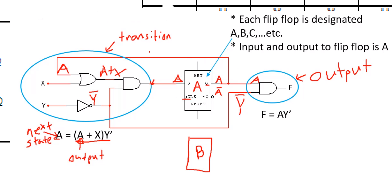
\includegraphics[width=14cm]{StateEquations1.png}\\
          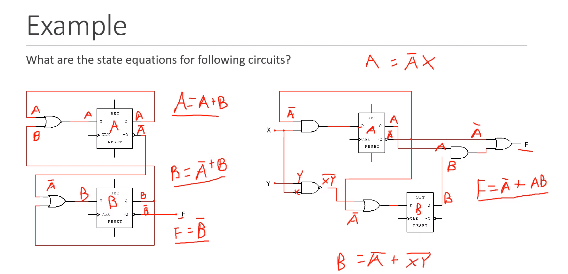
\includegraphics[width=15cm]{StateEquationsExamples.png}

\end{document}